\chapter{集合、关系与映射}
\label{chap:sets-functions-and-proofs}
\label{chap:sets-relations-maps}

设想一所学校开设四门课程，几名学生各自选了其中几门。拿到这份选课记录，会问：
哪些课程有人选，哪些课程两人都选了；某名学生与某门课程之间有没有选课联系；
怎样把每名学生对应到自己的选课；记录编号以后怎样汇总各门课的人数。
要据此推理和计算，需要先说清讨论哪些对象、对象之间有什么联系、
怎样把一个对象对应到另一个对象，以及怎样给一批对象编号并累计。

本章依次建立这些工具。集合规定讨论范围，集合运算组合成员条件；
关系把成对的联系记录为有序对的集合，其中等价关系用来分类，偏序用来比较；
映射是每个输入恰有一个输出的关系，单射、满射与双射刻画两个集合的元素能否逐一配对；
索引族用映射给一批对象编号，有限累计、数学归纳与递归处理有限多项的汇总和逐项生成。
下一章用双射和有限累计计数，第~\ref{chap:cardinality}章再用映射比较无限集合的大小。

\section{集合的定义与运算}
\label{sec:prelim-sets-relations-functions}

本节先说明怎样写出集合、怎样判断两个集合相等，再定义集合运算，
最后用已有集合构造幂集与笛卡尔积。

\subsection{集合的定义和描述}
\label{sec:prelim-set-definition}

\paragraph{集合与元素}
由一些确定的对象组成的整体称为\term{集合}（set），其中的对象称为它的元素；
“确定”是说任给一个对象，都能判断它是不是其中的元素。例如四门课程的编号组成集合$\{1,2,3,4\}$。
若$x$是集合$X$的元素，就说$x$属于$X$，记作$x\in X$；否则记作$x\notin X$。
集合只由它含有哪些元素决定：含有相同元素的两个集合相等，记作$X=Y$。
因此$\{1,2,3\}$、$\{3,2,1\}$与$\{1,1,2,3\}$是同一个集合。
不含任何元素的集合称为空集，记作$\varnothing$；只含一个元素$a$的集合$\{a\}$称为单元素集。

\paragraph{集合的描述}
列举法把元素逐个写在花括号中，例如$U=\{1,2,3,4\}$；
描述法写出挑选范围和所满足的条件，例如$U=\{i\in\mathbb Z:1\leq i\leq4\}$，
冒号读作“使得”，冒号前的$i\in\mathbb Z$表示从整数中挑选。挑选范围不能省略：
同一条件下从实数中挑选，得到的是区间$\{x\in\mathbb R:1\leq x\leq4\}=[1,4]$。
本书用$\mathbb N=\{0,1,2,\ldots\}$表示自然数集合，$\mathbb N_+=\{1,2,\ldots\}$表示正整数集合，
$\mathbb Z$、$\mathbb Q$和$\mathbb R$分别表示整数、有理数与实数集合；
区间$[a,b]$包含两个端点，$(a,b)$不含端点，$[a,b)$与$(a,b]$各只含一个端点。

\paragraph{子集}
若$A$的每个元素都属于$B$，就称$A$是$B$的子集（subset），记作$A\subseteq B$；
若还有$A\neq B$，就称$A$是$B$的真子集，记作$A\subsetneq B$。
属于与包含比较的对象不同：$1\in U$说的是编号$1$属于$U$，$\{1\}\subseteq U$说的是集合$\{1\}$包含于$U$；
$\{1,2\}\subseteq U$成立，$\{1,2\}\in U$却不成立，因为$U$的元素是编号而不是集合。
空集是任何集合的子集，因为“它的每个元素都属于$B$”无从违反。
由于集合只由元素决定，$A=B$当且仅当$A\subseteq B$且$B\subseteq A$；
证明集合相等时，常把等式拆成这两个包含分别验证，称为双向包含。

\subsection{集合的运算}
\label{sec:prelim-set-operations}

\paragraph{基本运算}
设甲、乙两名学生的选课分别是$C=\{1,2,3\}$与$D=\{2,3,4\}$，以全部课程$U=\{1,2,3,4\}$为全集。
合并名单、找共同课程、排除已知课程，分别对应下面的运算。
\begin{itemize}
 \item 并集：$X\cup Y=\{x:x\in X\text{ 或 }x\in Y\}$，“或”允许两个条件同时成立。例如$C\cup D=\{1,2,3,4\}$。
 \item 交集：$X\cap Y=\{x:x\in X\text{ 且 }x\in Y\}$，例如$C\cap D=\{2,3\}$。若$X\cap Y=\varnothing$，称$X$与$Y$不交。
 \item 差集：$X\setminus Y=\{x:x\in X\text{ 且 }x\notin Y\}$，例如$C\setminus D=\{1\}$，而$D\setminus C=\{4\}$。
 \item 对称差：$X\mathbin{\triangle}Y=(X\setminus Y)\cup(Y\setminus X)$，即恰好属于其中一个集合的元素，例如$C\mathbin{\triangle}D=\{1,4\}$。
 \item 补集：对全集$U$的子集$X$，$X^{\mathrm c}=U\setminus X$，例如$C^{\mathrm c}=\{4\}$。
       补集依赖全集：若全集换成$\{1,2,3,4,5\}$，$C$的补集就变成$\{4,5\}$。
\end{itemize}

\paragraph{运算律}
这些运算都由成员条件定义，运算律可以逐个元素核对。交与并满足交换律、结合律与分配律：
\begin{align*}
 X\cap Y&=Y\cap X,\\
 X\cup Y&=Y\cup X,\\
 (X\cap Y)\cap Z&=X\cap(Y\cap Z),\\
 (X\cup Y)\cup Z&=X\cup(Y\cup Z),\\
 X\cap(Y\cup Z)&=(X\cap Y)\cup(X\cap Z),\\
 X\cup(Y\cap Z)&=(X\cup Y)\cap(X\cup Z).
\end{align*}
前四式来自“且”“或”可以交换次序、改变组合方式。以第五式为例，左边要求$x\in X$，并且$x$属于$Y$或$Z$；
这恰好是说$x$同时属于$X$与$Y$，或者同时属于$X$与$Z$。
补集与交、并的关系由下面的定理给出。
\begin{theorem}[De Morgan律]
\label{thm:sets-de-morgan}
设$X,Y$是全集$U$的子集，则
\begin{equation}
 (X\cup Y)^{\mathrm c}=X^{\mathrm c}\cap Y^{\mathrm c},\qquad
 (X\cap Y)^{\mathrm c}=X^{\mathrm c}\cup Y^{\mathrm c}.
 \label{eq:prelim-de-morgan-two-sets}
\end{equation}
\end{theorem}
\begin{proof}
用双向包含证明第一式。若$u\in(X\cup Y)^{\mathrm c}$，则$u\notin X\cup Y$，因而$u\notin X$且$u\notin Y$，
即$u\in X^{\mathrm c}\cap Y^{\mathrm c}$。反过来，若$u\in X^{\mathrm c}\cap Y^{\mathrm c}$，则$u$既不属于$X$也不属于$Y$，
因而$u\notin X\cup Y$，即$u\in(X\cup Y)^{\mathrm c}$。
第二式同理：$u\notin X\cap Y$当且仅当$u\notin X$或$u\notin Y$，即$u\in X^{\mathrm c}\cup Y^{\mathrm c}$。
\end{proof}
第一式说的是，“不满足任何一个条件”与“每个条件都不满足”是同一件事；下一章计数违反限制的结果时要用到它。

\paragraph{差集的次序}
差集既没有交换律，也没有结合律。前面已有$C\setminus D\neq D\setminus C$；再取$E=\{1\}$，
则$(C\setminus D)\setminus E=\varnothing$，而$C\setminus(D\setminus E)=C\setminus D=\{1\}$。
所以连续求差时必须用括号标明先后。

\subsection{幂集、笛卡尔积与有序组}
\label{sec:sets-power-sets-products}

前面的运算得到的仍是原全集的子集。把一名学生的全部选课当成一个对象，
或者把“先选一门、再选一门”记录成一个对象，则需要构造新的集合。

\paragraph{幂集}
集合$X$的全部子集组成的集合称为$X$的\term{幂集}（power set），记作
\[
 \mathcal P(X)=\{A:A\subseteq X\}.
\]
例如$\mathcal P(\{1,2\})=\{\varnothing,\{1\},\{2\},\{1,2\}\}$，一名学生的全部可能选课就是课程集合的幂集。
幂集的元素是集合：$\{1\}\in\mathcal P(\{1,2\})$，而$1$不是$\mathcal P(\{1,2\})$的元素。
以集合为元素的集合也称为\term{集合族}（set family），它不必收集全部子集，例如$\{\{1\},\{2\}\}\subseteq\mathcal P(\{1,2\})$。
有限集合的幂集有多少个元素，留到下一章计算。

\paragraph{有序对与笛卡尔积}
集合不记录次序，有序对$(x,y)$则保留两个位置：$(x,y)=(x',y')$要求$x=x'$且$y=y'$。
所以$(1,2)\neq(2,1)$，而$\{1,2\}=\{2,1\}$；有序对还允许两个位置相同，如$(1,1)$。
第一个位置取自$X$、第二个位置取自$Y$的全部有序对组成\term{笛卡尔积}（Cartesian product）
\[
 X\times Y=\{(x,y):x\in X,\ y\in Y\}.
\]
例如$\{1,2\}\times\{a,b\}=\{(1,a),(1,b),(2,a),(2,b)\}$。当$X,Y$都非空且$X\neq Y$时，$X\times Y\neq Y\times X$。

一般地，有序$d$元组$(x_1,\ldots,x_d)$的第$i$个位置称为第$i$个坐标，两个$d$元组相等当且仅当对应坐标逐一相等。
第$i$个坐标取自$X_i$的全部$d$元组组成$X_1\times\cdots\times X_d$，各因子相同时记为$X^d$；
特别地，$\mathbb R^d$是全部有序$d$元实数组的集合，$\mathbb R^2$就是平面上点的坐标。
映射$(x_1,\ldots,x_d)\mapsto x_i$称为第$i$个投影。下一节的关系就是笛卡尔积的子集。

\section{关系与分类}
\label{sec:prelim-binary-relations}

“学生选了某门课”“$1$不大于$2$”“两个整数除以$3$的余数相同”，问的都是一对对象是否满足某个条件。
本节把这样的条件写成有序对的集合，研究关系的性质，再用两类特殊的关系分类和比较。

\subsection{二元关系及其性质}
\label{sec:prelim-binary-relation-definition}
\label{sec:prelim-relation-properties}

\paragraph{二元关系}
设三名学生$s_1,s_2,s_3$中，$s_1$选了课程$1,2,3$，$s_2$选了$2,3,4$，$s_3$没有选课。
选课情况是笛卡尔积$\{s_1,s_2,s_3\}\times\{1,2,3,4\}$的子集
\[
 R=\{(s_1,1),(s_1,2),(s_1,3),(s_2,2),(s_2,3),(s_2,4)\}.
\]
一般地，笛卡尔积的任一子集$R\subseteq X\times Y$称为$X$到$Y$的\term{二元关系}（binary relation），
写$xRy$表示$(x,y)\in R$；$X=Y$时称$R$为$X$上的关系。
至少与一个$y$有关系的$x$组成$R$的定义域，至少与一个$x$有关系的$y$组成$R$的值域；
上例的定义域是$\{s_1,s_2\}$，值域是全部四门课程。同一对集合之间可以有许多关系，空集和整个积也是关系；
关系也不要求每个$x$恰好对应一个$y$：$s_1$对应三门课，$s_3$一门也不对应。

\paragraph{关系的基本性质}
设$R$是集合$X$上的关系。
若每个$x\in X$都有$xRx$，称$R$具有\term{自反性}（reflexivity）；
若$xRy$总蕴含$yRx$，称$R$具有\term{对称性}（symmetry）；
若$xRy$与$yRx$只在$x=y$时同时成立，称$R$具有\term{反对称性}（antisymmetry）；
若$xRy$且$yRz$总蕴含$xRz$，称$R$具有\term{传递性}（transitivity）。

用三个熟悉的关系核对：
\begin{itemize}
 \item 相等关系：四种性质都有，因为它只关联同一个对象。
 \item 实数上的$\leq$：自反、反对称、传递，但不对称，因为$1\leq2$而$2\not\leq1$。
 \item 正整数上的整除$a\mid b$（存在正整数$c$使$b=ac$）：自反（$a=a\cdot1$）；传递（由$b=ac$、$e=bc'$得$e=a(cc')$）；
       反对称（$a\mid b$且$b\mid a$时$a\leq b\leq a$）；不对称。若放到非零整数上，$2\mid-2$且$-2\mid2$，反对称性不再成立。
\end{itemize}
最后一例说明，同一条规则是否具有某种性质，还取决于在哪个集合上讨论。

反对称性不是对称性的否定。若$xRy$成立时$yRx$总不成立，称$R$具有\term{非对称性}（asymmetry），
例如实数上的$<$；$\leq$不是非对称的，因为$1\leq1$。非对称关系一定反对称，
并且没有$x$满足$xRx$，即具有\term{反自反性}（irreflexivity）；反对称关系则允许$xRx$。

\paragraph{关系的闭包}
一个关系缺少某种性质时，可以补入必要的有序对。包含$R$、具有指定性质、并且在包含意义下最小的关系，
称为相应的\term{关系闭包}（closure of a relation）；“最小”是说任何包含$R$并具有该性质的关系都包含它。
反对称性不能靠补入有序对获得，因为已有的双向关联无法去掉。

自反闭包是$R\cup\{(x,x):x\in X\}$，对称闭包是$R\cup\{(y,x):(x,y)\in R\}$，补入的都是满足性质所必需的有序对。
例如$\{1,2,3\}$上的$\{(1,2),(2,3)\}$，自反闭包补入$(1,1),(2,2),(3,3)$，对称闭包补入$(2,1),(3,2)$。

传递闭包$R^+$规定：$xR^+y$当且仅当存在有限链$x=x_0,x_1,\ldots,x_n=y$（$n\geq1$），每一步都有$x_{k-1}Rx_k$。
两条链首尾相接仍是链，所以$R^+$传递；任何包含$R$的传递关系沿链使用传递性，都含有链的首尾对，所以$R^+$最小。
上例的传递闭包只需补入$(1,3)$。

\subsection{等价关系、划分与商集}
\label{sec:prelim-equivalence-relations}

\paragraph{等价关系}
按除以$3$的余数可以把整数分成三组。“分在同一组”这一关系应当满足：每个整数与自己同组；
$x$与$y$同组时$y$与$x$也同组；$x$与$y$、$y$与$z$分别同组时$x$与$z$也同组。这正是自反、对称与传递性。
\begin{definition}[等价关系]
\label{def:prelim-equivalence-relation}
设$R$是集合$X$上的关系。若$R$具有自反性、对称性与传递性，就称$R$为\term{等价关系}（equivalence relation）。
对$x\in X$，与$x$等价的元素组成$x$的\term{等价类}（equivalence class）
$[x]_R=\{y\in X:yRx\}$，$x$称为这个等价类的一个代表元。
\end{definition}
整数上的关系“$3$整除$x-y$”是等价关系：$x-x=0$；$x-y$是$3$的倍数时$y-x$也是；
$x-y$与$y-z$都是$3$的倍数时，它们的和$x-z$也是。它有三个等价类$[0],[1],[2]$，而$[3]=[0]$，
同一个等价类可以由不同的代表元写出。

\paragraph{等价类与划分}
若$X$的一族非空子集两两不交，并且它们的并等于$X$，就称这族子集为$X$的一个\term{划分}（partition）。
等价关系恰好给出划分。
\begin{theorem}[等价类构成划分]
\label{thm:sets-equivalence-partition}
设$R$是集合$X$上的等价关系，则全部等价类组成$X$的一个划分；并且对$x,y\in X$，或者$[x]_R=[y]_R$，或者$[x]_R\cap[y]_R=\varnothing$。
反过来，$X$的每个划分都由唯一的等价关系这样给出，即“属于同一块”。
\end{theorem}
\begin{proof}
由自反性，$x\in[x]_R$，所以每个等价类非空，并且各等价类的并是$X$。
设$z\in[x]_R\cap[y]_R$，即$zRx$且$zRy$。由对称性得$xRz$，再由传递性得$xRy$。
于是任取$u\in[x]_R$，由$uRx$与$xRy$得$uRy$，即$u\in[y]_R$，所以$[x]_R\subseteq[y]_R$；交换$x,y$得反向包含。
因此有公共元素的两个等价类相等，不同的等价类两两不交，全部等价类构成划分。
反过来，给定划分，令$xRy$当且仅当$x,y$属于同一块，三条性质直接成立，其等价类就是各块；
而任何以这些块为等价类的等价关系都必须如此定义，所以它唯一。
\end{proof}
因此，在同一个集合上给出等价关系与给出划分是同一件事的两种写法。

\paragraph{商集}
分组以后，常把每一组当作一个新对象。全部等价类组成的集合记为$X/R$，称为商集（quotient set）。
对整数按除以$3$的余数分组，商集是$\{[0],[1],[2]\}$；它的三个元素都是整数的子集，不是整数，
$0,1,2$只是用来写出它们的代表元。

正因为代表元只是记法，在商集上定义运算或映射时，必须检查结果不依赖代表元的选取。
例如规定$[a]+[b]=[a+b]$：若$a'\in[a]$、$b'\in[b]$，则$(a'+b')-(a+b)$仍是$3$的倍数，结果不变，所以这一加法有意义。
规定“$[a]$的奇偶性就是$a$的奇偶性”则不行：$0$与$3$代表同一个等价类，奇偶性却不同。

商集的元素也可以有几何含义。在平面上除原点以外的点中，规定$P\sim Q$当且仅当存在非零实数$c$使$P=cQ$，
这是等价关系，每个等价类是一条过原点的直线去掉原点；若只允许$c>0$，同一直线在原点两侧的部分分属两个类。
图~\ref{fig:vol1-add-equivalence-directions}比较这两种分类。
\begin{figure}[!htb]
  \centering
  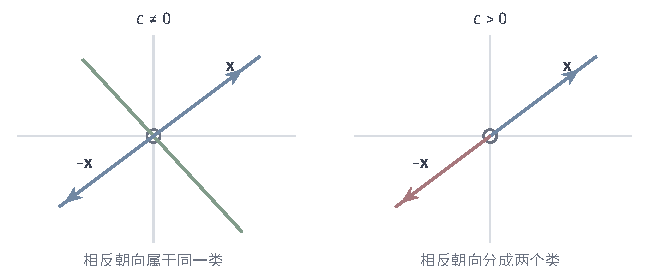
\includegraphics[width=112mm]{figures/01-mathematical-preliminaries-upper/00-shared/tikz/mathematical-language-combinatorics-analysis-optimization-comprehension-additions/equivalence-directions.pdf}
  \caption{平面中非原点的等价分类。每支箭头从原点指向一个点。左侧允许非零实比例，同一直线上的点属于同一类；右侧只允许正比例，同一直线的两侧分成蓝、红两类。绿色表示另一条直线上的类；空心原点不属于被分类的集合。}
  \label{fig:vol1-add-equivalence-directions}
\end{figure}

\subsection{偏序、全序与极值元素}
\label{sec:prelim-order-relations}

\paragraph{偏序与全序}
子集之间可以按包含比较，正整数之间可以按整除比较，但$\{1\}$与$\{2\}$互不包含，$2$与$3$互不整除。
这类比较关系都具有自反性、反对称性与传递性。
\begin{definition}[偏序关系]
\label{def:prelim-partial-order}
集合$X$上具有自反性、反对称性与传递性的关系称为\term{偏序关系}（partial order），常记作$\preceq$，
配备了偏序的集合记作$(X,\preceq)$。若$x\preceq y$与$y\preceq x$至少有一个成立，称$x$与$y$可比较。
若$X$中任意两个元素都可比较，则称$\preceq$为\term{全序}（total order）。
\end{definition}
实数上的$\leq$是全序，包含关系与整除关系只是偏序。

\paragraph{最小元与极小元}
设$A\subseteq X$非空。若$a\in A$满足$a\preceq b$对每个$b\in A$成立，称$a$为$A$的\term{最小元}（least element）；
若$b\preceq a$对每个$b\in A$成立，称$a$为\term{最大元}（greatest element）。
若$b\in A$且$b\preceq a$必有$b=a$，即$A$中没有比$a$更小的元素，称$a$为\term{极小元}（minimal element）；
若$b\in A$且$a\preceq b$必有$b=a$，称$a$为\term{极大元}（maximal element）。

在整除偏序下取$A=\{2,3,4,6\}$：$2,3$都是极小元，$4,6$都是极大元，但$A$没有最小元和最大元，因为$2$与$3$不可比，$4$与$6$也不可比。
最小元若存在则唯一：两个最小元彼此不大于对方，由反对称性相等。最小元一定是极小元；在全序中，极小元也是最小元。

\paragraph{上界与下界}
若$u\in X$满足$a\preceq u$对每个$a\in A$成立，称$u$为$A$的\term{上界}（upper bound）；
若$l\in X$满足$l\preceq a$对每个$a\in A$成立，称$l$为$A$的\term{下界}（lower bound）。
与最值元素不同，界不必属于$A$：上例中$12$是$A$的上界，$1$是下界，都不在$A$中。
全部上界中是否有最小的一个，一般偏序并不保证；实数集合的这一问题引出确界与完备性，见第~\ref{sec:prelim-optimal-values-errors}节。

\section{映射}
\label{sec:prelim-functions-value-ranges}

关系允许一个对象对应多个对象，也允许不对应任何对象。“每名学生的学号”“每个实数的平方”则要求每个输入恰好得到一个输出。
本节定义这种映射，研究像与原像，按能否逐一配对给映射分类，最后讨论复合与逆映射。

\subsection{映射、像与原像}
\label{sec:prelim-function-definition}

\paragraph{映射的定义}
设$X,Y$是两个集合。若$X$到$Y$的关系使每个$x\in X$恰好与一个$y\in Y$有关系，
就称它为$X$到$Y$的\term{映射}（map），也称\term{函数}（function），记作$f:X\to Y$；
与$x$对应的元素记作$f(x)$，记号$x\mapsto f(x)$读作“把$x$对应到$f(x)$”。
$X$称为定义域或源集，$Y$称为陪域或目标集，集合$\{(x,f(x)):x\in X\}$称为$f$的图像（graph）。
实际取得的输出组成$f(X)=\{f(x):x\in X\}$，称为值域或像集，它是目标集的子集。

上一节的选课关系不是映射：$s_1$对应三门课，$s_3$不对应任何课。实数上的$x\mapsto x^2$则是映射。

给出映射要同时说明源集、目标集和对应规则。同一规则$x\mapsto x^2$可以给出$\mathbb R\to\mathbb R$与$\mathbb R\to[0,\infty)$两个映射，
值域都是$[0,\infty)$，但前者的目标集中还有取不到的负数。两个映射相等，要求源集、目标集分别相同，且在每个输入处取值相同。
从$X$到$Y$的全部映射组成的集合记为$Y^X$，例如$\{0,1\}^{\{1,2\}}$有四个元素，由$(f(1),f(2))$的四种取值确定。

\paragraph{像与原像}
对映射$f:X\to Y$，可以问一组输入得到哪些输出，也可以问一组输出来自哪些输入。
对$A\subseteq X$与$B\subseteq Y$，分别定义$A$的像与$B$的\term{原像}（preimage）：
\begin{equation}
 f(A)=\{f(x):x\in A\}\subseteq Y,\qquad
 f^{-1}(B)=\{x\in X:f(x)\in B\}\subseteq X.
 \label{eq:prelim-preimage}
\end{equation}
对平方映射$f:\mathbb R\to\mathbb R$，$f(\{-2,1\})=\{1,4\}$，$f^{-1}(\{1\})=\{-1,1\}$，$f^{-1}([1,4])=[-2,-1]\cup[1,2]$，$f^{-1}(\{-1\})=\varnothing$。
原像是集合，可以含多个元素，也可以为空；记号$f^{-1}(B)$并不要求$f$有逆映射。
原像与集合运算相容：对$B,B'\subseteq Y$，
\begin{align*}
 f^{-1}(B\cup B')&=f^{-1}(B)\cup f^{-1}(B'),\\
 f^{-1}(B\cap B')&=f^{-1}(B)\cap f^{-1}(B'),\\
 f^{-1}(Y\setminus B)&=X\setminus f^{-1}(B).
\end{align*}
像只保持并，对交集一般只有$f(A\cap A')\subseteq f(A)\cap f(A')$。平方映射把$-1$与$1$都送到$1$，
于是$f(\{-1\}\cap\{1\})=\varnothing$，而$f(\{-1\})\cap f(\{1\})=\{1\}$。

\subsection{单射、满射与双射}
\label{sec:prelim-function-types}

对映射$f:X\to Y$，若不同输入的输出总不相同，即$f(x_1)=f(x_2)$必推出$x_1=x_2$，称$f$为\term{单射}（injection）；
若每个$y\in Y$都至少是一个输入的输出，即$f(X)=Y$，称$f$为\term{满射}（surjection）；
既单又满的映射称为\term{双射}（bijection）。

这些性质依赖源集和目标集。平方映射$\mathbb R\to\mathbb R$既不是单射也不是满射；
把目标集缩小为$[0,\infty)$，它成为满射；再把源集限制为$[0,\infty)$，它成为双射。
双射把两个集合的元素一一配对，说明它们“一样多”；单射把$X$的元素放进$Y$的不同位置，说明$X$“至多与$Y$一样多”。
下一章用双射计数，第~\ref{chap:cardinality}章用这两种比较研究无限集合。

\subsection{复合映射与逆映射}
\label{sec:prelim-map-operations}

\paragraph{复合与恒等映射}
对$f:X\to Y$与$g:Y\to Z$，定义\term{复合}（composition）映射$g\circ f:X\to Z$为
\[
 (g\circ f)(x)=g(f(x)).
\]
复合要求$f$的输出都在$g$的源集中；例如$g(u)=\sqrt u$定义在$[0,\infty)$上，$f(x)=x-1$只有限制在$x\geq1$上才能与它复合。

复合一般不能交换次序：$f(x)=x^2$、$g(x)=x+1$时，$(g\circ f)(1)=2$，而$(f\circ g)(1)=4$。

但复合满足结合律：对$h:Z\to W$，逐层代入得$(h\circ(g\circ f))(x)=h(g(f(x)))=((h\circ g)\circ f)(x)$，所以
\[
 h\circ(g\circ f)=(h\circ g)\circ f.
\]
单射的复合是单射，满射的复合是满射，因而双射的复合是双射。

映射$\operatorname{id}_X:X\to X$，$\operatorname{id}_X(x)=x$，称为恒等映射；对$f:X\to Y$有$f\circ\operatorname{id}_X=f=\operatorname{id}_Y\circ f$。
若先做一步、再做另一步的复合是恒等映射，第二步就撤销了第一步。

\paragraph{逆映射}
\phantomsection
\label{def:prelim-invertible-map}
撤销$f:X\to Y$，就是对每个$y\in Y$找回唯一的输入。若$f$是双射，满射保证这样的输入存在，单射保证它唯一；
把$y$对应到这个输入，得到$f$的逆映射（inverse map）$f^{-1}:Y\to X$，它满足
\[
 f^{-1}\circ f=\operatorname{id}_X,\qquad f\circ f^{-1}=\operatorname{id}_Y.
\]
反过来，若存在$h:Y\to X$使$h\circ f=\operatorname{id}_X$且$f\circ h=\operatorname{id}_Y$，则$f$是双射：
由$f(x_1)=f(x_2)$两边作用$h$得$x_1=x_2$；每个$y$都等于$f(h(y))$。
所以双射恰好是具有双侧逆映射的映射。例如$[0,\infty)\to[0,\infty)$的$x\mapsto x^2$的逆映射是$y\mapsto\sqrt y$。

逆映射与原像不同：原像对任何映射都有定义，作用在集合上；逆映射只对双射存在，作用在元素上。
对双射，$f^{-1}(\{y\})=\{f^{-1}(y)\}$，两者一致。图~\ref{fig:prelim-preimage-inverse}比较这两种反向操作。
若$f:X\to Y$与$g:Y\to Z$都是双射，则
\begin{equation}
 (g\circ f)^{-1}=f^{-1}\circ g^{-1},
 \label{eq:prelim-inverse-composition}
\end{equation}
因为由结合律$(f^{-1}\circ g^{-1})\circ(g\circ f)=f^{-1}\circ f=\operatorname{id}_X$，另一侧同理。
例如先平方、再加$1$把$x\geq0$送到$z=x^2+1$，撤销时先减$1$、再开平方。
后两章将反复用双射的复合换掉难数的集合、证明两个集合等势。

\begin{figure}[htbp]
  \centering
  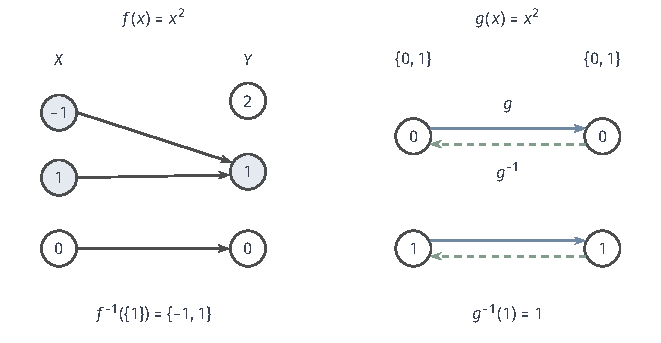
\includegraphics[width=112.0mm]{figures/01-mathematical-preliminaries-upper/01-mathematical-language-combinatorics-analysis-optimization/tikz/prelim-preimage-inverse/figure.pdf}
  \caption{原像与逆映射回答不同问题。左侧$f:\{-1,0,1\}\to\{0,1,2\}$按平方取值，
  标出的$1$有两个原输入，$2$没有原输入；原像$f^{-1}(\{1\})=\{-1,1\}$仍有定义。
  右侧将定义域与陪域都限制为$\{0,1\}$得到双射$g$，实线表示正向求值，虚线表示
  逆映射，因而$g^{-1}(1)=1$是一个元素。两侧均为精确的有限映射。}
  \label{fig:prelim-preimage-inverse}
\end{figure}

\section{索引族}
\label{sec:prelim-indices-sums-recurrences}

三次测验的得分是$1,1,4$，组成集合时只剩$\{1,4\}$，求总分时却要把两个$1$分别计入。
本节用映射给每次出现一个编号，再讨论一族集合的并与交、有限多个数的累计，以及归纳与递归。

\subsection{索引族的定义}
\label{sec:prelim-indexed-sequences}

\paragraph{索引族}
给每次测验一个编号，再为每个编号指定得分，就是一个映射。
\begin{definition}[索引族]
\label{def:prelim-indexed-family}
给定索引集合$I$和对象集合$X$，映射$a:I\to X$也称为以$I$为索引的\term{索引族}（indexed family），
把$a(i)$记作$a_i$，整个族记作$(a_i)_{i\in I}$。$i$称为指标，$a_i$称为指标$i$对应的对象。
\end{definition}
测验得分写成$a_1=1$、$a_2=1$、$a_3=4$。不同指标可以对应相同的对象，所以索引族与取值集合$\{a_i:i\in I\}=\{1,4\}$不同：
前者保留每一次出现，后者只记录出现过哪些值。

\paragraph{序列}
按正整数顺序索引的族称为序列（sequence）：只取$1,\ldots,n$时是有限序列，取全部正整数时是无限序列；
取值为实数的序列称为数列，例如$(1/n)_{n\geq1}$。从$0$开始编号时写$(a_n)_{n\geq0}$。
记录逐步更新的结果时，把第$t$步的结果记作$a^{(t)}$，用带括号的上标表示步数，以区别于幂$a^t$。

\paragraph{二维索引族与集合族}
两个指标共同指定一个对象时，得到二维索引族$(a_{i,j})_{(i,j)\in I\times J}$。
例如$a_{i,j}=3(i-1)+j$（$i=1,2$，$j=1,2,3$）排成两行$(1,2,3)$与$(4,5,6)$，固定$i$得到一行，固定$j$得到一列。
对象也可以是集合，例如三名学生的选课$(S_i)_{i\in\{1,2,3\}}$。这样的族记录的是每份选课，
不能与全部选课的并混为一谈：$S_1=\{1,2\}$、$S_2=\{2\}$时，并集$\{1,2\}$只记录哪些课程有人选过。

\subsection{集合族的运算}
\label{sec:prelim-indexed-set-operations}

给定全集$U$的子集族$(A_i)_{i\in I}$，“至少属于一个成员”和“属于每个成员”分别定义索引并与索引交：
\[
 \begin{aligned}
  \bigcup_{i\in I}A_i&=\{u\in U:\text{存在 }i\in I\text{ 使 }u\in A_i\},\\
  \bigcap_{i\in I}A_i&=\{u\in U:\text{对每个 }i\in I\text{ 都有 }u\in A_i\}.
 \end{aligned}
\]
$I=\{1,2\}$时回到$A_1\cup A_2$与$A_1\cap A_2$；$I=\mathbb N_+$时也写成$\bigcup_{n=1}^\infty A_n$与$\bigcap_{n=1}^\infty A_n$。
按定义，空族的交是全集$U$，空族的并是空集。De Morgan律对任意索引族同样成立：
\begin{equation}
 \Bigl(\bigcup_{i\in I}A_i\Bigr)^{\mathrm c}=\bigcap_{i\in I}A_i^{\mathrm c},\qquad
 \Bigl(\bigcap_{i\in I}A_i\Bigr)^{\mathrm c}=\bigcup_{i\in I}A_i^{\mathrm c},
 \label{eq:prelim-de-morgan-families}
\end{equation}
证明与定理~\ref{thm:sets-de-morgan}相同：不存在$i$使$u\in A_i$，就是对每个$i$都有$u\in A_i^{\mathrm c}$。

在$U=[0,1]$中取递增族$A_n=[1/n,1]$，则$\bigcup_{n\geq1}A_n=(0,1]$：每个$x>0$在$n\geq1/x$时属于$A_n$，而$0$不属于任何$A_n$。
取递减族$B_n=[0,1/n)$，则$\bigcap_{n\geq1}B_n=\{0\}$。成员都是区间，无限并却缺了端点，无限交只剩一个点；后面测量集合时还会遇到这类现象。

\subsection{有限累计}
\label{sec:prelim-finite-sums-products}

\paragraph{有限和与有限积}
对$n\geq1$个数$a_1,\ldots,a_n$，记
\[
 \sum_{i=1}^{n}a_i=a_1+\cdots+a_n,\qquad \prod_{i=1}^{n}a_i=a_1\cdots a_n.
\]
这两个记号只是有限次运算的缩写，可以逐项规定：$\sum_{i=1}^{n+1}a_i=\sum_{i=1}^na_i+a_{n+1}$，积同理。
逐项规定需要起点，约定空和为$0$、空积为$1$：
\[
 \sum_{i\in\varnothing}a_i=0,\qquad \prod_{i\in\varnothing}a_i=1,
\]
这样把一组项拆成两部分分别汇总时，即使一部分为空，结果也不变。
对有限索引集合$I$，也写$\sum_{i\in I}a_i$与$\prod_{i\in I}a_i$；这些记号在整数、有理数、实数中含义相同。

\paragraph{索引与有限换序}
求和变量的名称不影响结果：$\sum_{i=1}^na_i=\sum_{k=1}^na_k$，这里的$i$称为\term{哑索引}（dummy index）。
自由索引则留在结果中：在$b_j=\sum_{i=1}^{n}x_{i,j}$中，$j$须固定才知道汇总的是哪一列，
所以可以把$i$改为$k$，却不能只改右边的$j$，也不能把$i$改名为已占用的$j$。
平移哑索引时，范围要随之改写：$\sum_{n=1}^{N}b_{n+1}=\sum_{m=2}^{N+1}b_m$。

由加法、乘法的交换律、结合律与分配律，有限和满足线性关系
\[
 \sum_{i=1}^{n}(\alpha u_i+\beta v_i)=\alpha\sum_{i=1}^{n}u_i+\beta\sum_{i=1}^{n}v_i,
\]
有限积满足$\prod_{i=1}^n(a_ib_i)=\bigl(\prod_{i=1}^na_i\bigr)\bigl(\prod_{i=1}^nb_i\bigr)$与$\prod_{i=1}^n(ca_i)=c^n\prod_{i=1}^na_i$；
积没有线性关系，例如$(1+2)(3+4)\neq1\cdot3+2\cdot4$。结合平移与线性关系得到裂项求和：
\begin{equation}
 \sum_{n=1}^N(b_{n+1}-b_n)=\sum_{m=2}^{N+1}b_m-\sum_{n=1}^{N}b_n=b_{N+1}-b_1.
 \label{eq:prelim-telescoping-sum}
\end{equation}
例如由$\frac1{n(n+1)}=\frac1n-\frac1{n+1}$得$\sum_{n=1}^N\frac1{n(n+1)}=1-\frac1{N+1}$。

对二维有限数组$(a_{i,j})$，$i=1,\ldots,n$，$j=1,\ldots,d$，按行汇总与按列汇总相等：
\[
 \sum_{i=1}^{n}\sum_{j=1}^{d}a_{i,j}=\sum_{j=1}^{d}\sum_{i=1}^{n}a_{i,j},
\]
因为两边都把每个索引对恰好计入一次。内层范围依赖外层索引时，换序要重写范围，使遍历的仍是同一批索引对：
\begin{equation}
 \sum_{i=1}^{n}\sum_{j=1}^{i}a_{i,j}=\sum_{j=1}^{n}\sum_{i=j}^{n}a_{i,j},
 \label{eq:prelim-triangular-sum}
\end{equation}
两边都恰好遍历满足$1\leq j\leq i\leq n$的$(i,j)$；若把右边内层误写成$i=1,\ldots,n$，就会多算$j>i$的项。
这些换序依赖项数有限；无限多项的和要先用极限定义，不能由有限情形直接推广。

\subsection{数学归纳与递归}
\label{sec:prelim-recurrence-unrolling}

\paragraph{数学归纳}
设$\rho\neq1$，记$G_N=\sum_{n=0}^N\rho^n$（约定$\rho^0=1$）。由$G_0=1$、$G_1=\frac{1-\rho^2}{1-\rho}$、$G_2=\frac{1-\rho^3}{1-\rho}$，可以猜测
\begin{equation}
 \sum_{n=0}^N\rho^n=\frac{1-\rho^{N+1}}{1-\rho}\qquad(\rho\neq1),
 \qquad\sum_{n=0}^N1^n=N+1.
 \label{eq:prelim-finite-geometric-sum}
\end{equation}
验证前几项不能保证公式对每个$N$成立。\term{数学归纳法}（mathematical induction）给出证明方法：
要证明关于$N=0,1,2,\ldots$的命题$P(N)$全部成立，只需证明$P(0)$成立（归纳基础），
以及对每个$N\geq0$，由$P(N)$能推出$P(N+1)$（归纳步）；归纳步中假定成立的$P(N)$称为归纳假设。
对上式，$N=0$时两边都是$1$；若$G_N=\frac{1-\rho^{N+1}}{1-\rho}$，则
\[
 G_{N+1}=G_N+\rho^{N+1}=\frac{1-\rho^{N+1}+\rho^{N+1}-\rho^{N+2}}{1-\rho}=\frac{1-\rho^{N+2}}{1-\rho}.
\]
所以公式对每个$N$成立；$\rho=1$时每项都是$1$，和为$N+1$。

有时证明$P(N+1)$要用到此前的全部命题。强归纳法规定：若$P(0)$成立，并且对每个$N\geq0$，
由$P(0),\ldots,P(N)$全部成立能推出$P(N+1)$，则$P(N)$对一切$N$成立；把命题换成“$P(0),\ldots,P(N)$都成立”，它就回到普通归纳。
例如每个大于$1$的整数$m$都是素数之积：$m$是素数时成立；否则$m=ab$，$1<a,b<m$，由较早阶段的结论，$a,b$都是素数之积，于是$m$也是。

\paragraph{递归}
给定集合$X$、初值$x_0\in X$与更新映射$T:X\to X$，规定
\[
 x_{t+1}=T(x_t),\qquad t=0,1,2,\ldots,
\]
这种用已有的项确定下一项的定义方式称为\term{递推}（recurrence），也称递归定义；有限和的逐项规定就是一例。
递推确实确定了唯一的序列：称满足$y_0=x_0$且$y_{k+1}=T(y_k)$（$k<n$）的$(y_0,\ldots,y_n)$为长度$n+1$的初段，
对$n$归纳可知每个长度的初段恰有一个，且较短的初段是较长初段的开头部分；
令$x_n$为长度$n+1$的初段的末项即得所求序列，而任何满足递推的序列的前$n+1$项都是初段，因而与之相同。

递推定义对象，归纳证明它的性质。例如等比递推
\begin{equation}
 e^{(t+1)}=\rho e^{(t)},\qquad e^{(0)}=e_0,\qquad t=0,1,\ldots
 \label{eq:prelim-geometric-recurrence}
\end{equation}
在$e_0=8$、$\rho=1/2$时给出$8,4,2,1,\ldots$，提示通项$e^{(t)}=\rho^te_0$；
归纳验证：$t=0$时成立，若$e^{(t)}=\rho^te_0$，则$e^{(t+1)}=\rho^{t+1}e_0$。等差递推$a^{(t+1)}=a^{(t)}+d$同理得$a^{(t)}=a_0+td$。
由$|e^{(t+1)}|=|\rho|\,|e^{(t)}|$，$|\rho|<1$时非零项的绝对值逐步缩小，$|\rho|>1$时逐步放大，$\rho=-1$时大小不变、符号交替。
$t$无限增大时这些数怎样变化，要到第~\ref{chap:function-limits}章用极限回答。

\section{本章小结}
\label{sec:prelim-sets-functions-summary}

集合由元素决定，集合相等可以用双向包含证明，运算律与De Morgan律都能逐个元素核对，差集则没有交换律和结合律；
幂集收集全部子集，笛卡尔积记录有次序的多次选择。关系是笛卡尔积的子集：等价关系与划分是同一结构的两种写法，
商集上的运算必须与代表元无关；偏序允许对象互不可比，最小元与极小元、界与最值要分别判断。

映射要求每个输入恰有一个输出。原像保持并、交与补，像一般不保持交；单射、满射与双射依赖源集和目标集，
双射恰好具有双侧逆映射，逆映射作用于元素，原像作用于集合。索引族保留每次出现的编号，
有限和与有限积换序时须遍历同一批项；递推定义序列，归纳证明它的性质。

全章要分清对象本身与它的编号（索引）、等价类与代表元、映射与表示它的规则表达式。
下一章用双射把有限集合与$\{1,\ldots,n\}$配对，借助分类、分步、对应和递推计数；
第~\ref{chap:cardinality}章再用单射和双射比较无限集合的大小。实值函数的运算、确界和极限从第~\ref{chap:function-limits}章开始讨论。
